\documentclass{literature}

\title{Exploring the physical properties of high redshift galaxies with KMOS}
\subtitle{First year report}
\author{Owen J. Turner}
\authoremail{turner@roe.ac.uk}
\supervisor{Dr. Michele Cirasuolo}
\supervisoremail{ciras@roe.ac.uk}
\slugheader{First year report}
\slugauthor{Owen J. Turner}
\logo{/Users/owenturner/Documents/PhD/KMOS/Latex/Literature_Review/UoEcrest.pdf}
\graphicspath{{Users/}{owenturner/}{Documents/}{PhD/}{KMOS/}{Latex/}{Literature_Review/}{Figures/}}
\abstract{This is a first year report detailing what I've been up to over my first 9 months as a PhD student and laying out the path that will be taken from here going forwards. }
\setcounter{secnumdepth}{4}


\begin{document}

\coverpage



%%%%%%%%%%%%%%%%%%%%%%%%%%%%%%%%%%%%%%%%%%%%%%%%%%%%%%%%%%%%%%%%%%%%%%%%%%%%%%%%%%%%%%%%%%%%%%%%%%%%%%%%%%%%%%%%%%%%%%


\section{Introduction}\label{sec:Intro}
The physical processes which govern the formation and evolution of high redshift galaxies are representative of a time when the universe was most active. It is the gas within these galaxies which is the driving force behind galaxy evolution, and there are various tools provided by the latest generation of telescope which allow astronomers to explore the properties of this gas. \\ 



Throughout this first year report, I will give a brief overview of how to go between telescope data and the physical properties of a galaxy, indicating the literature surrounding this in section \ref{sec:background}. Section \ref{subsec:current_int} gives an overview of the telescopes 
routinely collecting the spectra of high redshift galaxies, highlighting the wavelength ranges in which their detectors operate and whether 
they have the capacity for integral field spectroscopy. Section \ref{sec:KMOS} focusses specifically on the specifications of KMOS and the key science drivers motivating research with this instrument. 





\section{Background}\label{sec:background}
mini lit review introduction. Set the context 

\citep{Troncoso_2014}, \citep{Maiolino2008}, \citep{Cullen2014}, \citep{Kewley2002}, \citep{Kennicutt_2012}, \citep{Tremonti2004} \citep{Brinchmann2004} \citep{Savaglio2005} \citep{Erb_2006} \citep{Kewley_2008} \citep{ForsterSchreiber2009} \citep{Steidel2014}
Major themes are: 

\begin{itemize}
	\item The need for detailed measurements of high-z galaxies with integral field spectrometers 
	\item a description of available IFS at different portions of the spectrum, kmos optimised for Halpha at z3
	\item Dust
	\item Measurement of abundance 
	\item photoionization models and population synthesis
	\item morphology 
	\item gas dynamics, outflows and the connection between this and evolution 
	\item flux data cubes 
	\item the mass metallicity relation and the fmr 
	\item use of abundance techniques described by cullen 
\end{itemize}

Plots will be: 

\begin{itemize}
	\item peak of SFRd curve 
	\item m-z relation at different epochs 
	\item Attempts to force the strong lines to be equal 
	\item Gradients in physical properties from Troncoso
	\item Some spectra -  
	\item look at all the plots from your other document 
\end{itemize}



M-Z graphs at different redshifts and FMR graphs to illustrate the point. Wanting to confirm the shape of both at redshift 3, or actually looking at the M-Z relation at different points throughout the galaxy - i.e. does the centre of the galaxy follow a different M-Z relation to the outskirts of the galaxy. 

\subsection{Measuring Flux}
Dust extinction, calzetti curves etc. 

 

\subsubsection{Slit Loss Corrections}
Corrections to H$\alpha$ lines fluxes due to slit losses. A particular redshift corresponds to an angular diameter distance, and the physical size of the galaxy subtends a particular angular size at this distance. The telescope being used has an entrance slit of a particular angular size. The point spread function of a galaxy is spread over a larger angular size by Gaussian seeing of a given FWHM which depends on the atmospheric conditions at the time of observation. It is possible that the resultant PSF has FWHM larger than the entrance slit, and so a certain fraction of the light emitted by the galaxy is falling outside of the slit. Corrections for this effect have a particular bearing on emission line analysis, as they are required to ensure accurate ratios between lines taken through different photometric filters and observed under different weather conditions \citep{Reddy2015}. Typically an estimate of the fraction of light lost is found by modelling the light profile of the galaxy, convolving with the seeing disk and integrating through the slit. Is this something which is relevant for KMOS?     


\subsubsection{Dust and Extinction}
section 2.3.2 of Steidel and Calzetti 2000 and Draine 2003. Attenuation curves for the Milky Way and for other galaxies - how consistent is the Calzetti curve as a) a function of galaxy type and b) a function of redshift 


\subsection{Measuring Stellar Masses}
Stellar masses are routinely estimated using stellar population synthesis models, which construct the SEDs of populations of stars. The shape of these SEDs depend on the physical properties of the galaxy, i.e. age, metallicity, redshift and stellar mass. A grid of model SEDs is constructed by varying these physical properties in the population synthesis, and the values are constrained through comparison to an observed SED. The most widely used models are those of Bruzual and Charlot \citep{Bruzual2003} (BC03). \\      
Typically, spectroscopic surveys will target well studied fields to make use of ancillary photometric data. These data preferably cover as wide a region of the spectrum as possible, to provide the information required to break degeneracies between physical properties, such as age and metallicity. As a concrete example, consider the procedure described in Steidel et al. (2014) \citep{Steidel2014}, where stellar masses are estimated for a sample of $z \sim 2$ galaxies. The galaxies have been observed in three optical filters (\textit{$U_{n}GR$}), the near-IR  $ J $ and $ K_{s}$ bands, the HST WFC3-IR F160W filter and the Spitzer/IRAC 3.6$\mu m$ and 4.5$\mu m$ beams. These data cover both the region of the spectrum where rest-frame starlight is emitted directly, and where starlight absorbed by dust is re-radiated. The BC03 models are used to fit the observed SED and stellar masses are inferred by assuming a Chabrier IMF \citep{Chabrier2003}, with estimated uncertainties in log($M_{*} /M_{\odot}$) of $\pm 0.1-0.2 $ dex.    


\subsection{Measuring Star Formation Rates}
Throughout their lifetimes, galaxies convert bound gas into stars, and do so at a varying rate. The star formation rate is an indicator of the efficiency with which stellar mass is being built up within a galaxy, and is dependent upon galaxy type, environment and cosmic epoch. Observations have revealed that most stars form within galaxies that follow a relatively tight SFR-M$_{*}$ `Main Sequence'. The existence of this sequence suggests that the evolution of the global Star Formation History (SFH) of the universe is determined by a balance between gas accretion and feedback to the IGM, such as stellar winds, supernovae shocks and AGN activity. Understanding these processes which regulate the gas volume and composition within a galaxy, and seemingly drive the changes in star formation rates over time is a fundamental aspect of galaxy evolution. \\ 
Here an overview of the observational methods employed to measure the SFRs of galaxies is given. 
Sections \ref{subsubsec:uv_continuum} - \ref{subsubsec:comp} describe the individual SFR tracers, the motivation behind their use and the benefits and downfalls of applying them independently. Underpinning all of these techniques are Stellar Population Synthesis (SPS) codes, which use the equations of stellar evolution to model the light emitted by a population of stars at different ages. The spectrum of a galaxy is determined by the ratio of early-type to late-type stars, and so the observed colour of a galaxy contains information about the star formation over the most recent stage of the galaxy's history. By modelling galaxy colours as a function of SFR, age, composition and IMF, SPS codes provide a calibration between the observed luminosity of a particular SFR tracer and the SFR of the galaxy. Section \ref{subsubsec:gsfh} will summarise the now consistent picture of the global SFH of the universe, highlighting the peak period of star formation at $z \sim 2$.  \\ 

The advent of NIR integral-field spectrographs on 8-10m class telescopes has paved the way for studying spatially resolved SFRs within galaxies during the time when the universe was at its most active. Spatially resolved spectroscopy is crucial for uncovering the dependency of SFR upon environment, rather than making an assumption that the galaxy properties are similar across its spatial extent and deriving a holistic SFR. Section \ref{subsubsec:spat_res} will discuss this in more detail, focussing on the opportunities presented by these instruments and the observational challenges which must be overcome to reach these goals.     


\subsubsection{The UV continuum}\label{subsubsec:uv_continuum}
The wavelength range 1200-2500\AA is longward of the Lyman-continuum break and bluewards of the contaminating flux emitted by older stellar populations. The near-UV continuum emission of galaxies in the range traces the photospheric emission of young stars and is thus one of the most direct methods of measuring galaxy SFRs. Advantages, disadvantages, current calibrations\\ 

For extragalactic studies, this method has been revolutionised by the launch of Galaxy Evolution Explorer mission (GALEX, \citep{Martin2005}). GALEX imaged two thirds of the sky in near-UV (230nm) and far-UV (155nm) channels, providing integrated measurements of distant galaxies and resolved mapping for our nearest external galaxies. The impact of this is the recovery of UV flux measurements for hundreds of thousands of galaxies, which can be used to calibrate the relationship between luminosity and SFR and also to provide fresh data to constrain the relationship between the UV spectral slope and dust attenuation.      

\subsubsection{Infrared Emission}\label{subsubsec:ifrared}


\subsubsection{Emission Line Tracers}\label{subsubsec:em_lines}

\subsubsection{Radio and X-ray Tracers}\label{subsubsec:rad_x}


\subsubsection{Composite Multiwavelength Tracers}\label{subsubsec:comp}

\begin{figure}[!htp]
\centering
\includegraphics[width=0.8\textwidth]{comp_tracers.png}
\caption{\footnotesize{\emph{Calibrated SFR tracers using combined multi-wavelength tracers}}}
\label{fig:comp_convert}
\end{figure} 



\begin{figure}[!htp]
\centering
\includegraphics[width=0.8\textwidth]{convert.png}
\caption{\footnotesize{\emph{Conversion factors between observed luminosity and SFR for different tracers.}}}
\label{fig:convert}
\end{figure} 


In sum, Kennicutt and Evans \citep{Kennicutt_2012} tabulate the conversion between luminosity and SFR for each of the tracers listed above. Figure \ref{fig:convert} lists the units of the observed luminosities, $L_{x}$, in the different wavebands, and the value of the constant, $C_{x}$, used to convert to SFR. This conversion is given by Equation ~\ref{eq:convert} below. 

\begin{equation} \label{eq:convert}	
	log\dot{M_{*}}(M_{\odot}year^{-1}) = logL_{x} - logC_{x}
\end{equation}



Gas flows both to and from the IGM in high redshift galaxies are crucial to allowing for, and limiting, the very high star formation rates and accompanying metal production during the peak epoch of galaxy formation. \\

\subsubsection{The Global Star Formation History}\label{subsubsec:gsfh}
Overall, having a handle on the global SFR of the universe at different epochs tells us about the activity of the universe at these times. We appear to live at a time which is much less active than in the past, with stars forming at a peak rate that is 9 times higher than is seen today.\citep{Madau_2014}

\begin{figure}[!htp]
\centering
\includegraphics[width=0.8\textwidth]{sfh.png}
\caption{\footnotesize{\emph{The history of cosmic star formation from a) FUV b) IR and c) FUV + IR.}}}
\label{fig:sfh}
\end{figure} 


\subsubsection{Spatially Resolved SFRs}\label{subsubsec:spat_res}


\subsection{Measuring Cosmic Abundance}\label{subsec:abundance}
Giant HII regions were the first indicators of the gas phase abundance of galaxies, and of abundance gradients across the face of these galaxies \citep{Searle1971}, \citep{Shields1974}. Many other abundance indicators have been used since then, including supernova remnants, stellar clusters and AGB stars. HII regions are relatively easy to observe, and the interpretation of their spectra is straightforward, and so these remain the favoured tool for abundance determination.  \\


Description of the physical process which excites atoms and causes them to emit the `forbidden' lines - gas rarefied enough \\


Chemical abundances derived in low metallicity regions are generally considered reliable, given that the spectroscopy is deep enough to allow for an accurate measurement of forbidden line ratios such as [OIII] $\lambda 4363/5007$, and hence the electron temperature $T_{e}$. DESCRIPTION OF THE DIRECT METHOD. This is the so-called `direct $T_{e}$' method, and requires high quality data which are sensitive to weak, fordibben transitions. The method becomes rapidly more challenging at higher redshifts, where the HII regions are fainter and the required forbidden lines are redshifted into regions of the spectrum plagued by much higher terrestial background. \\   






At these redshifts, astronomers rely upon the suite of statistical strong-line methods to measure HII region abundances. \\

Description of the main methods (Either from Hughes thesis or from Kewley and Ellison) \\ 

However, the metallicities derived using separate strong line indicators are often not in agreement, with discrepancies of up to a factor of 3 for different strong-line indicators applied to the same set of data. This is mainly due to some of the techniques being calibrated using theoretical models and some empirically with observations of electron temperature sensitive emisison lines \citep{Stasinska2005}. There have been attempts to force the strong-line methods to yield the same metallicites when applied to large samples of high redshift galaxies, by converting measurements to the same metallicity `baseline' \citep{Kewley_2008}, \citep{Kewley2002}, \citep{Maiolino2008}

`It is a separate issue as to whether the re-normalisation of strong-line techniques can (or should) be applied to samples of high redshift galaxies - clearly this is a desirable property but has not yet been clearly demonstrated. The root of the problem is that for this to be allowed, the physics of high redshift HII regions would have to resemble the physics of local star-forming galaxies. If there are any significant physical differences, blind application of local calibrations will introduce systematics in inferred metallicity'. Perhaps the most challenging situation is the comparison of metallicities derived with one set of strong-line indicators in a particular redshift range with those based on a different set of lines at a second redshift. 




\subsection{Measuring Gas Dynamics}\label{subsec:Gas-Dynamics}

These are some of the 

\subsection{BPT Diagram}\label{subsec:BPT-diagram}
The `Baldwin, Phillips, Terlevich' (BPT) diagram is a plane defined by the strong emission line ratios [OIII]/H $\beta$ and [NII] / $H\alpha$. Perhaps the most remarkable aspect of the BPT diagram is the tight locus along which most local star-forming galaxies are found, sometimes referred to as the `HII region abundance sequence'. Tremonti et al. constructed the BPT diagram for a sample of $> 50,000$ local SDSS star-forming galaxies, shown as the grey points in Figure \ref{fig:steidel_bpt}, revealing two branches, the first of which is the locus of star-forming galaxies and the second is the subset of galaxies with AGN activity. Galaxies hosting AGN have much harder UV spectra, the effect of which is to boost the ratio OIII/H $\beta$ relative to NII/H $\alpha$. The BPT diagram is therefore a useful diagnostic test for the presence of these galaxies, which are excluded from abundance analyses as their strong line ratios are unlikely to be related to stellar processes. \\ 


A crucial goal of high redshift galaxy abudance measurement is to understand the physical origins of the difference in position between the $z \sim 0$ and $z > 1$ locus of star forming galaxies in the BPT diagram. Figure \ref{fig:steidel_bpt} shows the BPT diagram for a sample of local SDSS galaxies \citep{Tremonti2004} and for a sample of galaxies from KBSS-MOSFIRE with $z \sim 2.3$. Clearly there is a vertical offset between the two populations  
relating to the appropriateness of using locally calibrated strong-line abundance diagnostics at high redshift. 

Reasons for the difference (all from the steidel paper end of section 4)
\begin{itemize}
	\item Harder radiation field 
	\item higher ionisation parameter 
	\item weaker dependence of N/O on O/H
\end{itemize}
combine to give a weaker dependence of the observed strong lines on the abundance - i.e. tie in the BPT shifts to the abundance measurement consequences. 
must also mention \citep{Kewley2013} once you've read.1/4

\begin{figure}[!htp]
\centering
\includegraphics[width=0.8\textwidth]{steidel_bpt.png}
\caption{\footnotesize{\emph{The `BPT' diagram shows the position of star-forming galaxies in the [OIII]/H $\beta$ vs. [NII] / $H\alpha$ plane. This particular figure, taken from Steidel et al. 2014 \citep{Steidel2014}, shows the locus of $z \sim 2.3$ KBSS MOSFIRE star forming galaxies (green) relative to the SDSS $z \sim 0$ galaxies (grey) \citep{Tremonti2004}. The BPT diagram is also used as an AGN diagnostic, with galaxies hosting active AGN being identified as having unusually large [OIII]/H $\beta$ relative to [NII] / $H\alpha$.}}}
\label{fig:steidel_bpt}
\end{figure} 

\subsection{Mass-Metallicity relationship and evolution}\label{subsec:MZ-relation}

Main points are the flattening of the MZR above a characteristic $M_{*}$ in the low redshift universe, any functional fits to the data take this into account, analogous to the $L_{*}$ in a luminosity function. \\ 
The drop in metallicity for a given stellar mass when moving to higher redshift and the physical explanation for this \\ 
The difficulty and danger of comparing the MZR at different redshifts due to the points above about strong-line indicators perhaps not being sensitive to the actual oxygen abundance at high redshift. Evolution of the gas content within galaxies. 
\citep{Savaglio2005}, \citep{Maiolino2008}, \citep{Erb_2006}, \citep{Tremonti2004}, \citep{Kewley2013}

\begin{figure}[!htp]
\centering
\subfloat[]{\includegraphics[width=0.32\textwidth]{tremonti_mzr.png}}
\subfloat[]{\includegraphics[width=0.32\textwidth]{steidel_mzr.png}}
\subfloat[]{\includegraphics[width=0.32\textwidth]{Maiolino_mzr.png}}
\caption{\footnotesize{\emph{}}}
\label{fig:steidel_mzr}
\end{figure}





\subsection{Fundamental metallicity relationship and evolution}

\subsection{Current multi-object and integral field spectrographs}\label{subsec:current_int}
	
Emphasis is now being placed on the role Multi-Object Spectrographs (MOSs) play in revealing the properties of object populations. For years, single object spectrographs have revealed a huge amount about the properties of small numbers of these objects. However, detailed knowledge of the behaviours of object populations is difficult to grasp without the statistical power of larger collections of spectra, which sample different object environments and reveal a wider spread in galaxy physical properties. Particularly for ground based observations in parts of the spectrum strongly affected by atmospheric effects, some of the most exciting applications of spectroscopy involve very long integration times, even on 10m telescopes. By simultaneously collecting spectra for many objects, MOSs promise to collect much larger samples of spectra from which more robust conclusions can be drawn. \\

Integral Field Spectrographs (IFSs), or spectrographs equipped with Integral Field Units (IFUs) combine the capacity for imaging and for spectroscopy. The result is resolved spectroscopy, in which a galaxy image is split into a grid, and each segment of the grid is dispersed using a grating to obtain a spectrum. This collection of spectra for a single galaxy image is called a datacube, which contains information about how the physical properties of the galaxy change across its radial extent. Studies involving resolved spectroscopy are crucial for understanding the gas, and by extension galaxy, evolution, through looking at abundance and SFR gradients and by directly examining the gas dynamics. The current observational benchmark is the combination of both integral field and multi-object spectroscopy with a single instrument, providing large samples of resolved spectra. This is the optimal research tool for developing an understanding of the physical processes driving galaxy formation and evolution. At increasingly high redshifts, the rest-frame optical emission lines used to measure abundance and trace gas velocity are shifted to longer wavelengths. As a result, to develop a coherent view of galaxy evolution throughout the cosmic epochs it is necessary to have instruments sensitive across the optical and near-IR regions of the spectrum.  \\ 

Sections \ref{subsubsec:MUSE} - \ref{subsubsec:VIMOS} highlight spectrographs which are currently operational with either integral field or multi-object capabilities, indicating the passbands in which they are sensitive. In section \ref{sec:KMOS} focus turns to the K-band Multi-Object Spectrograph (KMOS), which is the instrument used throughout this work.     

\subsubsection{MUSE}\label{subsubsec:MUSE}
The Multi-Unit Spectroscopic Explorer (MUSE) \citep{Bacon2010} is an optical mutli-object integral field spectrograph operating at the Nasmyth focus of Unit Telescope 4 (UT4), part of ESO's Very Large Telescope (VLT) array in Chile. 	

\subsubsection{MOSFIRE}\label{subsubsec:MOSFIRE}
The Multi-Object Spectrometer For Infra-Red Exploration (MOSFIRE) \citep{McLean2012} is a multi-object spectrograph for the Keck observatory in Hawaii. KBSS-MOSFIRE is a deep near-IR survey covering 15 fields of the Keck Baryonic Structure Survey (KBSS), specifically targeting the redshift range $2.0 < z < 2.6$, a range in which a relatively complete set of the rest-optical nebular lines fall fortuitously within the near-IR atmospheric windows for ground based spectroscopy. As a result, this survey is optimised for collecting spectra for and examining the properties of star forming galaxies during the peak of the SFRd curve. On top of this, the MOSFIRE Deep Evolution field (MOSDEF) \citep{Kriek2014}  aims to collect $\sim 1500$ rest-frame optical spectra in three well studied Cosmic Assembly Near-Infrared Deep Extragalactic Legacy Survey (CANDELS) \citep{Grogin2011} fields.

\subsubsection{SINFONI}\label{subsubsec:SINFONI}
The Spectrograph for INtegral Field Observations in the Near Infrared (SINFONI) \citep{Eisenhauer2003} is an integral field spectrograph operating at the Cassegrain focus of UT4 at the VLT array. The spectroscopic imaging survey in the near-infrared with SINFONI (SINS) collected the largest sample of spatially resolved gas kinematics, morphologies and physical properties of star forming galaxies at $z \sim 1-3$ \citep{ForsterSchreiber2009}. 

\subsubsection{VIMOS}\label{subsubsec:VIMOS}
The Visible Multi-Object Spectrograph (VIMOS) \citep{LeFevre2003} is a wide field imager and multi-object spectrograph mounted on the Nasmyth focus of UT3 at the VLT array. The Vimos VLT Deep Survey (VVDS) collected thousands of spectra from the Chandra Deep Field South area, \citep{LeFvre2004}, \citep{LeFevre2005}, which are crucial in there own right, but also act as important calibration data for photometric redshift techniques \citep{Ilbert2006}.

\subsubsection{OSIRIS}\label{subsubsec:OSIRIS}


\subsubsection{LUCIFER}\label{LUCIFER}

\subsubsection{GMOS}
Gemini observatory 

\subsubsection{MaNGA}\label{subsubsec:MaNGA}
Mapping Nearby GAlaxies is a new survey at Apache Point Observatory as part of the Sloan Digital Sky Survey IV (SDSS-IV), with the aim of obtaining integral-field spectroscopy for an unprecendented sample of 10000 nearby galaxies. MaNGA's key goals are to understand the `life cycle' of present day galaxies from imprinted clues of their birth and assembly, through their ongoing growth via star formation and merging, to their death from quenching at late times. To achieve these goals, MaNGA will channel the impressive capabilities of the SDSS-III BOSS spectrographs in a fundamentally new direction by marshaling the unique power of 2D spectroscopy

\subsubsection{MOONS}\label{subsubsec:MOONS}
Throughout this work, I have been using data collected by KMOS, which combines multi-object and integral field spectroscopy in the near-IR. 

\section{KMOS}\label{sec:KMOS}
As detailed in the above sections there is an expanding selection of impressive instrumentation available both for multi-object and for integral field spectroscopy. It is worthwhile to focus on where KMOS fits in to the big picture. Section \ref{subsec:instrument} provides a description of the instrument design and the crucial science drivers motivating its construction and section \ref{sec:reduction} describes the key recipes of the reduction pipeline required to turn raw images into reconstructed data cubes. 

\subsection{Specification, science drivers and context}\label{subsec:instrument}
The details of the physical processes driving galaxy formation and evolution in the first few billion years after the big bang remain elusive. The ideal set of operational capabilities for an instrument seeking to shed light on these topics are as follows. 
\begin{itemize}
	\item The ability to collect spectra for many objects simultaneously; a statistically robust sample will be difficult to assemble with single object IFUs alone 
	\item The ability to obtain more than just integrated or one dimensional information, since forming galaxies are often observed to have complex morphologies 
	\item Sufficient resolving power to detect the relatively small differences in velocity observed in galaxy rotation curves
	\item The flexibility to target objects clustered together in small areas of the total field of view 
	\item The ability to observe well studied optical features at high redshift in the near-IR Y, J, H and K-band atmospheric windows    
\end{itemize}

These are in essence the key features of KMOS, which is a near-IR multi-object integral field spectrograph operating with 24 configurable pickoff arms in the Nasmyth focal plane. These arms position mirrors at user specified locations, which feeds the light through to 24 image slicer IFUs that position each sub-field into 14 identical slices with 14 spatial pixels along each slice. Light from the IFUs is then dispered by three identical cryogenic grating spectrometers to generate 14x14 spectra for each sub-field, with the dispersed light reaching three identical 2kx2k Hawaii 2RG HgCdTe detectors. Each spatial pixel corresponds to 0.2$^{\prime \prime}$, giving each IFU a 2.8$^{\prime \prime}$x2.8$^{\prime \prime}$ sub-field. Each arm patrols the 7.2$^{\prime}$ diameter of the total field of view of the telescope. This system offers significant advantages over multi-slit spectrographs, because of the reduced slit contention in crowded fields, and the sensitivty of the pickoff arms to galaxy morphology and orientation. KMOS operates in 5 near-IR bands, these being the IZ, YJ, H, K and HK, with varying spectral resolution between these \citep{Sharples2005}. \\ 

KMOS is perfectly equipped to map variations in star formation histories, merger rates and dynamical masses across a wide range of redshifts and environments, these being probes of the history of galaxy evolution in the universe.  
 

\subsection{Data Reduction Pipeline}\label{sec:reduction}
By virtue of being a multi-object integral field spectrometer with 24 configurable IFUs and over 4000 spectra per exposure, the raw data taken by KMOS, and hence the reduction pipeline, are complex. Fortunately, ESO has made available the Software Package for Astronomial Reductions with KMOS (SPARK) \citep{Davies2013}, for carrying out the bulk of this reduction. Included in this package are recipes for processing dark frames and flatfields, for wavelength calibration of the spectral pixels in the chosen waveband using a set of arc frames and static calibration files, flux calibration with standard star images and a set of science reduction recipes to reconstruct and combine data cubes using the above calibrations. At the end of each night, the relevant set of calibration images are taken at six different rotator angles, to allow for the closest match to the rotation angle of the data as possible. \\ 

Thus far this pipeline has been incredibly useful, and each recipe contains a set of configurable options to give the user more control over how the reduction is carried out. There are however some steps missing from the reduction pipeline which can improve the quality of the resultant data and hence the accuracy of the spectra extracted from the data cubes. One of my tasks has been to make these additions to the pipeline, describe in section \ref{subsec:kmos_pipeline}.  




\section{Work since September 2014}\label{sec:work}
This section gives overview of the work completed since the beginning of my PhD in September. To supplement the tasks described in the following subsections, background reading for the above literature review was carried out continuously throughout this period. The notes from this reading, as well as notes from each meeting with Michele, have been recorded in an electronic journal. 

\subsection{Cosmology calculator}\label{subsec:cosmo_calc}
As an introduction to coding with Python, and to provide an important tool for the extraction of physical properties from spectra, I wrote a program to compute the age, light travel time, comoving volume, comoving radial distance, angular diameter distance and luminosity distance, $D_{L}$, at redshift z, given the set of cosmological parameters $(H_{O}, \Omega _{M}, \Omega _{V})$. This is in the same vein as Ned Wright's Cosmology Calculator \citep{Wright2006}, and makes use of the equations provided in the summary of distance measures in cosmology by David Hogg \citep{Hogg1999}. Figure \ref{fig:cosmo_calc} plots these distances in units of the Hubble distance $D_{H} = \frac{c}{H_{0}}$, against redshift for a flat cosmology with $H_{0} = 70kms^{-1}Mpc^{-1}$, $\Omega _{M} = 0.3$, $\Omega _{V} = 0.7$.  

\begin{figure}[!htp]
\centering
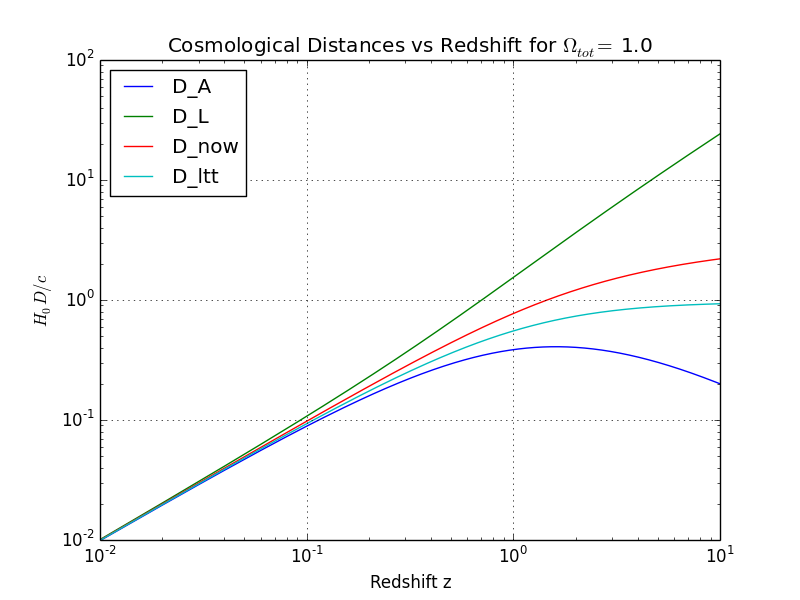
\includegraphics[width=0.6\textwidth]{cosmo_dist.png}
\caption{\footnotesize{\emph{Output from the cosmology calculator program, showing divergence between the different distance measures with increasing redshift. The dark blue line shows the angular diameter distance, the green line shows the luminosity distance, the red line shows the radial comoving distance and the light blue line the light travel distance.}}}
\label{fig:cosmo_calc}
\end{figure}    

\subsection{Analysing reduced SDSS spectra}\label{subsec:sdss_spec}
To motivate the development of a bespoke KMOS pipeline, we decided first to analyse the pre-reduced spectra of a set of normal, local SDSS galaxies. This back-to-front approach demonstrates the type of analysis that will be applied to KMOS galaxy spectra, albeit with significantly higher signal-to-noise than will be possible with the $z\sim 3$ KMOS galaxy sample. 
Broadly this section can be split into two categories, the first dealing with the extraction of emission line fluxes by fitting gaussians to the spectral locations of the emission lines. The second is the application of calibrated formulae to the parameters of the fitted gaussians to recover the physical properties of the galaxies. These categories are now discussed in turn.  

\subsubsection{Extracting Emission Line Fluxes}\label{subsub:ex_em}   
The reduced spectra were extracted from the `specObj' table of SDSS DR10 via SQL search. The SDSS database is a particularly useful testbed, as the optical emission line parameters as well as global galaxy properties derived from these are listed here and can be used for comparison.  The first stage of the analysis is to fit and subtract the continuum emission of the galaxy, here carried out in two separate ways. Either a third order polynomial is fit to the data, with emission lines masked, or a moving average is applied to match the continuum with a higher level of detail. Typically the simple polynomial fit provided emission line fluxes which matched the SDSS values more closely, and this is what is used throughout this section. Following continuum subtraction, it is necessary to know the redshift of the galaxy in order to determine the spectral locations of the emission line peaks. Here, and as would be the case in many other situations, the redshift of the galaxies is known and the wavelengths of the emission lines can be determined using the simple relation: 

\begin{equation}
\label{eq:redshift}
	\lambda _{peak} = (1 + z)\lambda _{vacuum}
\end{equation}

In the more general case where redshift is unknown, synthetic galaxy spectra can be used to give an indication of the expected shape of the galaxy SED. Early, intermediate and late-type synthetic spectra are plotted in Figure \ref{fig:temp_spec}. By shifting these synthetic spectra along a grid of redshift values and computing the cross correlation coefficient, $\rho$, with the observed spectrum after each shift, three separate $\rho$ arrays are determined. The maximum value of $\rho$ in each array corresponds to the redshift at which the observed and shifted template spectra best resemble each other. For these SDSS spectra, the late-type galaxy template produces by far the highest values of $\rho$ and the inferred galaxy redshift is always taken from this. An example of a cross correlation `power' plot against redshift for an observed spectrum and the shifted late-type template is shown in Figure \ref{fig:cross_cor}. The redshift value $z = 0.138$ agrees well with the value reported in the database.    \\ 




\begin{figure}[!htp]
\centering
\includegraphics[width=0.8\textwidth]{temp_spec.png}
\caption{\footnotesize{\emph{The synthetic spectra of early, intermediate and late-type galaxies, used for cross-correlation and redshift determination. Emission feautures becoming more prominent with age, as ionised nebulae become enriched by successive generations of star formation.}}}
\label{fig:temp_spec}
\end{figure} 

\begin{figure}[!htp]
\centering
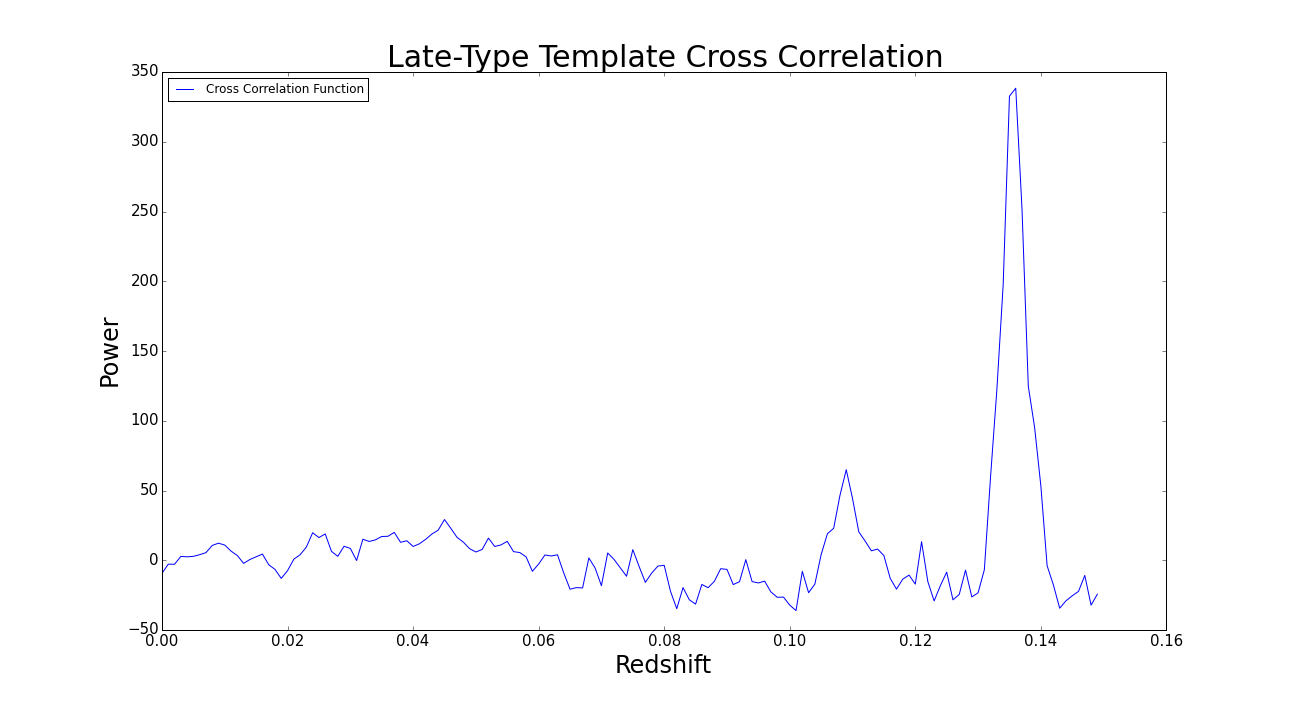
\includegraphics[width=0.8\textwidth]{Cross_corr.png}
\caption{\footnotesize{\emph{The cross correlation `power' is plotted against the grid of redshift values passed to the function, showing a clear peak at $z\sim 0.138$. This is a relatively easy procedure for such high quality spectra with prominent emission lines, becoming increasingly difficult to gain enough signal as redshift increases. }}}
\label{fig:cross_cor}
\end{figure} 

Once the redshift of the galaxy has been determined, equation \ref{eq:redshift} gives the recipe for finding the wavelengths of the peaks of the emission lines. A table of the known vacuum wavelengths for H$\beta$, [OIII]$\lambda 4959$, [OIII]$\lambda 5007$, H$\alpha$, [NII]$\lambda 6585$, [SII]$\lambda 6718$ and [SII]$\lambda 6732$ was used to find the observed wavelengths for each galaxy, and a gaussian function is fit to the data surrounding these emission line peaks in turn by fixing the central value. The area underneath the gaussian is the flux of that emission line and is also used to find the line equivalent width, whereas the width of the gaussian is used to determine the FWHM of the line, important for velocity measurements. A plot is made of the whole spectrum, with each emission line overlaid in red, to check the quality of these fits. Figure \ref{fig:fitted_spec} (a) gives an example of this, with panel (b) showing the wavelength region surrounding $H\alpha$ and confirming that the fitted gaussians closely match the shape of the emission lines.\\    

\begin{figure}[!htp]
\centering
\subfloat[]{\includegraphics[width=0.5\textwidth]{fitted_spectrum_full.png}}
\subfloat[]{\includegraphics[width=0.5\textwidth]{fitted_spectrum_part.png}}
\caption{\footnotesize{\emph{An example of one of the SDSS spectra for a $z\sim 0.14$ galaxy. Panel (a) shows the galaxy spectrum in blue, with the fitted gaussians overlaid in red. Panel (b) shows the same with an expanded view of the region $7400-7700\AA$, encompassing the $H\alpha$, $[NII]\lambda 6585$, $[SII]\lambda 6718$ and $[SII]\lambda 6732$ emission lines, shifted in wavelength by the factor $(1 + z)$. Plot (b) clearly demonstrates the high quality of the fit.}}}
\label{fig:fitted_spec}
\end{figure}



\subsubsection{Recovering Physical Properties}
After recovering line fluxes from the galaxy spectra, these can be converted to line luminosities using the luminosity distance, $D_{L}$, to the galaxy at redshift z computed with the cosmology calculator. For example, the luminosity of H$\alpha$ at redshift z, recovered from flux F($H\alpha$) is given by: 

\begin{equation}
\label{eq:flux-lum}
 	L(H\alpha) = 4\pi D_{L}^{2} F(H\alpha)
\end{equation} 

As mentioned in section \ref{subsubsec:em_lines}, H$\alpha$ is a particularly sensitive tracer of the instantaneous star formation rate, as only the most massive, and hence short lived, stars contribute significantly to the ionising photon flux. Using the relation provided in Kennicutt and Evans \citep{Kennicutt_2012}: 

\begin{equation}
 	\label{eq:halpha_sfr}
 	SFR(H\alpha) = log_{10}(L(H\alpha)) - 41.27
 \end{equation} 

an estimation of the SFR in each galaxy is be found. Also, using the PP04 \citep{Pettini_2004} and KD02 \citep{Kewley2002} abundance indicators (Equations \ref{eq:PP04} and \ref{eq:KD02} respectively), two separate estimations of the metal abundance are found. The PP04 indicator is found to agree relatively well with the SDSS oxygen abundance, but as described in \ref{subsec:abundance} there are discrepancies between the abundances reported from different indicators.  

\begin{equation}
	\label{eq:PP04}
	12 + log(O/H) = 9.12 + (0.73\frac{F([NII]\lambda 6585)}{F(H\alpha)})
\end{equation}

\begin{equation}
	\label{eq:KD02}
	12 + log(O/H) = 8.73 - (0.32\frac{F([OIII]\lambda 5007)F(H\alpha)}{F([NII]\lambda 6585)F(H\beta}))	
\end{equation}

As a final test of the accuracy of the emission line fluxes extracted from the SDSS spectra, a BPT diagram was plotted for a sample of 50,000 test galaxies in Figure \ref{fig:owen_bpt}. These data are a subset of the grey points in Figure \ref{fig:steidel_bpt} and the distributions closely resemble one another. The subset of galaxies with higher ionisation parameter are clearly seen as those with higher $\frac{[OIII]}{H\beta}$ for given $\frac{[NII]}{H\alpha}$.


\begin{figure}[!htp]
\centering
\includegraphics[width=0.7\textwidth]{bpt_owen.png}
\caption{\footnotesize{\emph{The BPT AGN diagnostic diagram recovered from applying the gaussian fitting procedure described above for a sample of 50,000 galaxies extracted from the specPhoto table of SDSS DR10. There is clear bimodality in the diagram, reflecting the ionisation state of galaxies with and without AGN.}}}
\label{fig:owen_bpt}
\end{figure}    

It would have been interesting to investigate stellar masses recovered from SPS modelling and recover the local MZ-relationship as well as the local SFR vs. $M_{*}$ curve, but we decided not to pursue stellar masses at this stage as this was more an introduction to the topic than a rigorous analysis. \\ 

It is likely that the  spectrum fitting strategy will have to be significantly aletered when moving to higher redshifts, fainter galaxies and lower S/N, but this was helpful for learning the general principles involved in extracting fluxes and galaxy physical properties from pre-reduced spectra. We finished this section towards the middle of December, turning attention to KMOS and the reduction pipeline at the end of December and after the Christmas break.   

\subsection{Additions to the KMOS reduction pipeline}\label{subsec:kmos_pipeline}

As described in section \ref{subsec:kmos_pipeline}, following the recipes supplied in the ESO reduction pipeline allows the user to process raw object images into fully reduced data cubes. However, the `out of the box' pipeline skips several steps which can greatly increase the quality of the reconstructed data cubes. The importance of these steps is amplified during the reduction of high redshift galaxy images, where the signal to noise ratio is significantly lower. It is important to tease as much information out from the data as possible at these redshifts, especially when measuring the strengths of nebular emission lines. Ground based near-IR spectroscopy is plagued by telluric contamination, and so to extract reliable information from galaxy images, sky-subtraction must be performed as accurately as possible. The additions made to the ESO pipeline focus on improving the sky-subtraction process prior to science reconstruction, and correcting the infrared detectors for read noise effects. These additions are decsribed below.  \\ 
The overarching goal at this stage is to produce an automated pipeline which reliably extracts as much information as possible from the KMOS high redshift galaxy images. 

\subsubsection{Read noise}





\subsubsection{Object and sky image misalignment} 


\subsubsection{OH Emission and Sky Subtraction}

Emission lines produced by the OH radical dominate near-IR spectra, appearing between 0.61 - 2.62 $\mu m$ and with fluxes several orders of magnitude larger than other sky emission. These are produced by Meinel rotation-vibration transitions of the OH molecule, and appear in distinct bandings across the near-IR spectral range, as shown in Figure \ref{fig:sky_spec}. As a result, the removal of OH lines is an essential stage in the processing of near-IR data, with images of blank patches of sky being taken and then subtracted from the `object' images. Waves in the upper atmosphere cause a strong time dependence in both the absolute and relative intensities of these emission lines, complicating the removal process. For a clean subtraction, the flux of the OH lines in the sky and object images would have to vary by much less than 1 percent; yet the lines can vary significantly on time-scales of only a few minutes and often exposures times longer than this are required to achieve adequate S/N. To further complicate the subtraction process, manufacturing variations between instrument elements, and even small amounts of spectral flexure in the instrument during rotation can leave significant `P-Cygni' shaped residuals in the spectrum when a sky frame is subtracted. \\ 
So one cannot simply take the sky spectrum in one spatial pixel and subtract it from another, and for the reasons above, despite the rotation-vibration transitions of OH being very well understood \citep{Osterbrock1996}, attempts to generate and subtract synthetic OH spectra inevitably fail due to instrumental limitations and the time variation of OH emission.On a positive note, these lines serve as useful reference points for wavelength calibration of astronomical spectra, and near-IR sky emission line maps have been created to aid in the identification of these lines \citep{Rousselot2000}. \\ 

Discussing the rather complicated topic of IFS sky-subtraction \citep{AllingtonSmith1998a}, alternative method described by Davies \citep{Davies2007}.

 

\begin{figure}[!htp]
\centering
\includegraphics[width=0.8\textwidth]{sky_spectrum.png}
\caption{\footnotesize{\emph{A plot of the OH emission dominating the 1-1.4$\mu m$ region of the spectrum, extracted from a YJ-band KMOS skycube. The rotation-vibration bands of the OH molecule are clearly seen. These are extremely strong features, peaking at almost 5000 counts $s^{-1}$, orders of magnitude above the object flux.}}}
\label{fig:sky_spec}
\end{figure}

\begin{figure}[!htp]
\centering
\includegraphics[width=0.7\textwidth]{KMOS_SPEC_OBS258_0009_Corrected110_temp_spline3_CorrelationGraph.png}
\caption{\footnotesize{\emph{A contour plot for $\rho$ computed for the grid of x, y shift values passed to Pyraf imshift. The contours are centred on the maximum value of $\rho$, this corresponding to the shift values which best align the object and sky images. The contours are drawn at $\rho _{max} - 0.25\sigma$, $\rho _{max} - 0.75\sigma$ and $\rho _{max} - 1.5\sigma$ and indicate the presence of a global maximum, suggesting unique `best' shift values $\Delta x$ and $\Delta y$.}}}
\label{fig:rho_plot}
\end{figure}

\section{Planned projects}\label{sec:projects}
\subsection{The physical properties of galaxies at z = 3}
\subsubsection{Directly observing emission lines required for direct metallicity measurement}




\subsection{Searching for CIII Emission}




\subsection{Spectroscopic Confirmation of LAEs at z=7-8}

%%%%%%%%%%%%%%%%%%%%%%%%%%%%%%%%%%%%%%%%%%%%%%%%%%%%%%%%%%%%%%%%%%%%%%%%%%%%%%%%%%%%%%%%%%%%%%%%%%%%%%%%%%%%%%%%%%%%%%%%

\clearpage 
\bibliographystyle{apj.bst}
%\bibliography{/usr/local/texlive/texmf-local/bibtex/bib/ojt.bib}
\bibliography{/Users/owenturner/Documents/PhD/KMOS/Latex/Bibtex/library.bib}

\end{document}
